\chapter{Ergebnisse}
\label{sec:ergebnisse}

Im folgenden Protokollabschnitt werden die Versuchsergebnisse der Versuchsdurchführung präsentiert.
\vspace*{-3.5mm}

\section{Sedimentationsverhalten}
\section{Absetzvolumen}
\section{Trockensubstanz TS}
\section{organische Trockensubstanz oTS}
\section{chemischer Sauerstoffbedarf CSB}
\section{biologischer Sauerstoffbedarf BSB$_5$}

\newpage

\section{Gegenüberstellung der Mindestanforderungen für das Einleiten kommunaler Abwässer in einen Vorfluter der GK 5 mit den Abwasserproben}
Die Referenzwerte der Mindestanforderungen für das Einleiten kommunaler Abwässer in den Vorfluter der Größenklasse 5 sind im Anhang von \cite[S. 29]{Skript} zu finden.
\vspace*{-2.5mm}
\renewcommand{\arraystretch}{1.2}
\begin{table}[h!]
	\centering
	\caption{Tabellarischer Vergleich der Messwerte mit den Mindestanforderungen für das Einleiten kommunaler Abwässer in den Vorfluter der GK 5}
	\label{tab_vgl}
	%\resizebox{10cm}{!}{
	\begin{tabulary}{1.2\textwidth}{l|C|C|C}
		\hline
		Werte in \si{\milli\gram\per\liter} & \textbf{$NH_4^+-N$} & \textbf{$N_{ges}$}&\textbf{$P_{ges}$}\\
		\hline
		\textbf{Grenzwert} & \textbf{10} & \textbf{13} & \textbf{1} \\
		\hline
		Probe 1 & {\footnotesize kein Messwert\protect\footnotemark[5]} & 108 & {\footnotesize kein Messwert\protect\footnotemark[5]} \\
		Probe 2 & 1,3 & 0,77 & 3,9 \\
		Probe 3 & 0,6 & 2,18 & 8,8 \\
		\hline
	\end{tabulary}
	%}
\end{table}
\FloatBarrier

\begin{figure}[h!]
	\begin{tikzpicture}
	\selectcolormodel{gray}
	\begin{axis}[
	xbar=1pt,% space of 0pt between adjacent bars
	bar width=7,
	width=15cm,
	height=7cm,
	%minor y tick num=4,
	xmax=110,xmin=0,
	x tick label style={/pgf/number format/.cd,%
		scaled x ticks = false,
		set decimal separator={,},
		fixed},
	symbolic y coords={Probe 3,Probe 2,Probe 1\protect\footnotemark[5],max. für GK 5},
	ytick=data,
	%legend style={at={(0.5,-0.15)},
	%	anchor=north,legend columns=-1},
	xtick={0,10,...,110},
	grid=major,
	xlabel=Gehalt in  \si{\milli\gram\per\liter},
	%enlargelimits=0.15,
	%postaction={pattern=north east lines}
	]
	%NH4-N
	\addplot[pattern=north east lines] coordinates {
		(0,Probe 1\protect\footnotemark[5]) (1.3,Probe 2) (0.6,Probe 3) (10,max. für GK 5)
	};
	%N gesamt
	\addplot coordinates {
		(108,Probe 1\protect\footnotemark[5]) (0.77,Probe 2) (2.18,Probe 3) (13,max. für GK 5)
	};
	%P gesamt
	\addplot[fill=black] coordinates {
		(0,Probe 1\protect\footnotemark[5]) (3.9,Probe 2) (8.8,Probe 3) (1,max. für GK 5) 
	};
	\legend{$NH_4-N$,$N_{ges}$,$P_{ges}$}
	\end{axis}
	\end{tikzpicture}
	\caption{Vergleich mit Mindestanforderungen für das Einleiten kommunaler Abwässer in den Vorfluter der GK 5 für die Abwasserproben 1 bis 3}
	\label{Balkendiagramm}
\end{figure}
\FloatBarrier
\footnotetext[5]{kein Messwert für Phosphat- bzw. Ammoniumgehalt vorhanden}

\newpage

\section{Gegenüberstellung der durchschnittlichen Beschaffenheit von häuslichem Abwasser mit den Abwasserproben}

Um die Messwerte des Versuches mit häuslichem Abwasser gegenüberzustellen wird die Tabelle Tab. \ref{tab:komm} (siehe \cite[S. 29]{Skript}) genutzt.

\vspace*{-2.5mm}
\renewcommand{\arraystretch}{1.2}
\begin{table}[h!]
	\centering
	\caption[Tabellenausschnitt zur durchschnittlichen Beschaffenheit von häuslichem Abwasser]{Tabellenausschnitt zur durchschnittlichen Beschaffenheit von häuslichem Abwasser \cite[S. 29]{Skript}}
	\label{tab:komm}
	%\resizebox{10cm}{!}{
	\begin{tabulary}{1.2\textwidth}{l|C|C|C|C}
	\textbf{Kriterium} & \textbf{Maßeinheit} &\multicolumn{3}{c}{\textbf{Belastungsgrad}}\\
	\hline
			&		&	gering&mittel &stark\\
	\hline
	pH-Wert	& - & 6,6&7,6&,8,6\\
	$N_{ges}$&	\si{\milli \gram \per \liter} & 20&50&85\\
	$P_{ges}$&	\si{\milli \gram \per \liter} & 7&20&30\\
	\end{tabulary}
	%}
\end{table}
\FloatBarrier


\begin{figure}[h!]
	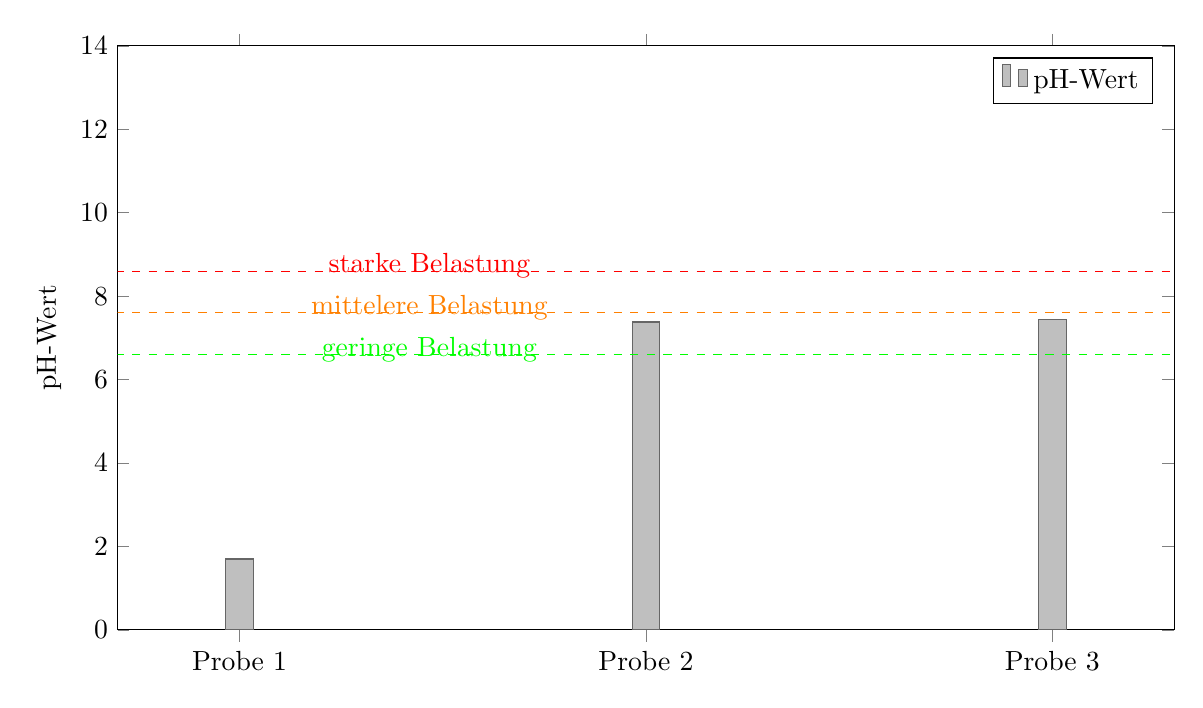
\begin{tikzpicture}
	\begin{axis}[
	%x tick label style={
	%	/pgf/number format/1000 sep=},
	xtick = data,
	ylabel=pH-Wert,
   	enlarge x limits=0.15,
	ybar,
	ymin = 0,
	ymax = 14,
	bar width=10pt,
	width=15cm,
	height=9cm,
	symbolic x coords={0,Probe 1, Probe 2,Probe 3,2,1},
	]
	\addplot[fill=gray!50,draw=black!60] coordinates {(Probe 1,1.7) (Probe 2,7.38) (Probe 3,7.44)};
	\addplot[green,sharp plot,update limits=false, dashed] 
	coordinates {(0,6.6) (1,6.6)} 
	node[above] at (axis cs:Probe 2,6.2) {\hspace*{-5.5cm}geringe Belastung};
	\addplot[orange,sharp plot,update limits=false, dashed] 
	coordinates {(0,7.6) (1,7.6)} 
	node[above] at (axis cs:Probe 2,7.2) {\hspace*{-5.5cm}mittelere Belastung};
	\addplot[red,sharp plot,update limits=false, dashed] 
	coordinates {(0,8.6) (1,8.6)} 
	node[above] at (axis cs:Probe 2,8.2) {\hspace*{-5.5cm}starke Belastung};
	\legend{pH-Wert}
	\end{axis}
	\end{tikzpicture}
	\caption{pH-Wert-Beschaffenheit der Abwasserproben 1 bis 3}
	\label{ph}
\end{figure}
\FloatBarrier

\newpage

\begin{figure}[h!]
	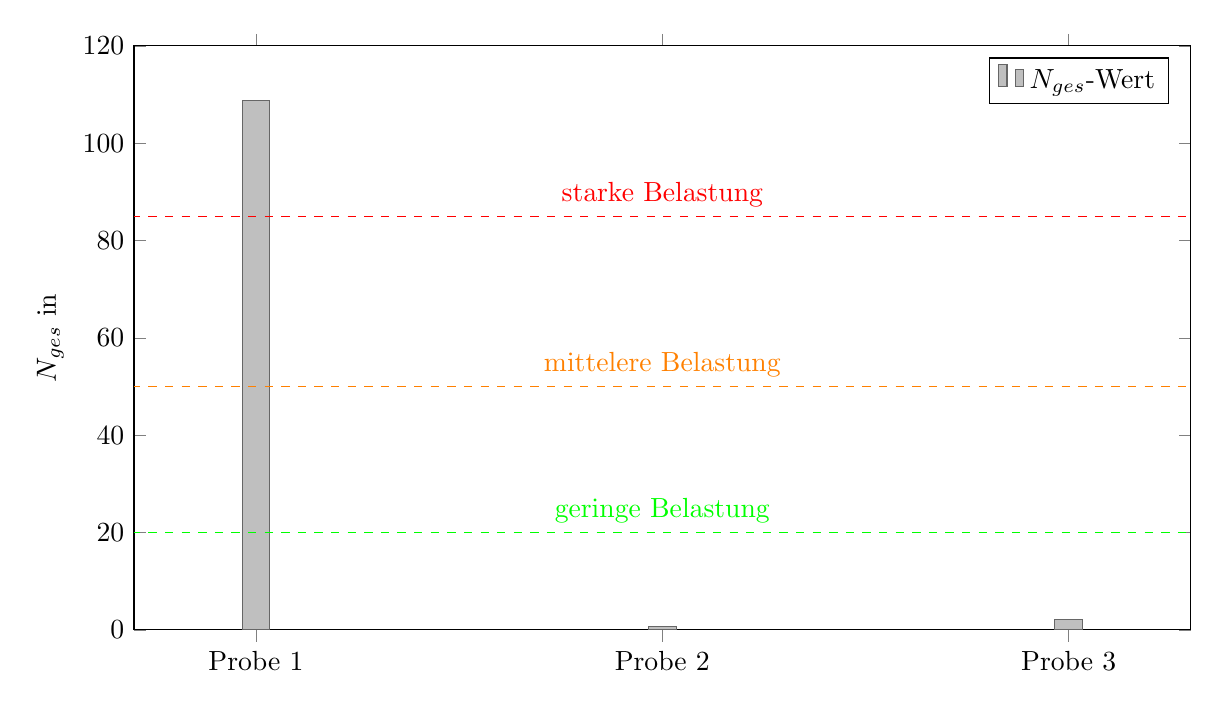
\begin{tikzpicture}
	\begin{axis}[
	%x tick label style={
	%	/pgf/number format/1000 sep=},
	xtick = data,
	ylabel=$N_{ges}$ in \si{\milli \gram \per \liter},
	enlarge x limits=0.15,
	ybar,
	ymin = 0,
	ymax = 120,
	bar width=10pt,
	width=15cm,
	height=9cm,
	symbolic x coords={0,Probe 1, Probe 2,Probe 3,2,1},
	]
	\addplot[fill=gray!50,draw=black!60] coordinates {(Probe 1,108.7) (Probe 2,0.77) (Probe 3,2.18)};
	\addplot[green,sharp plot,update limits=false, dashed] 
	coordinates {(0,20) (1,20)} 
	node[above] at (axis cs:Probe 2,20) {geringe Belastung};
	\addplot[orange,sharp plot,update limits=false, dashed] 
	coordinates {(0,50) (1,50)} 
	node[above] at (axis cs:Probe 2,50) {mittelere Belastung};
	\addplot[red,sharp plot,update limits=false, dashed] 
	coordinates {(0,85) (1,85)} 
	node[above] at (axis cs:Probe 2,85) {starke Belastung};
	\legend{$N_{ges}$-Wert}
	\end{axis}
	\end{tikzpicture}
	\caption{$N_{ges}$-Beschaffenheit der Abwasserproben 1 bis 3}
	\label{nges}
\end{figure}
\FloatBarrier

\vspace*{3cm}

\begin{figure}[h!]
	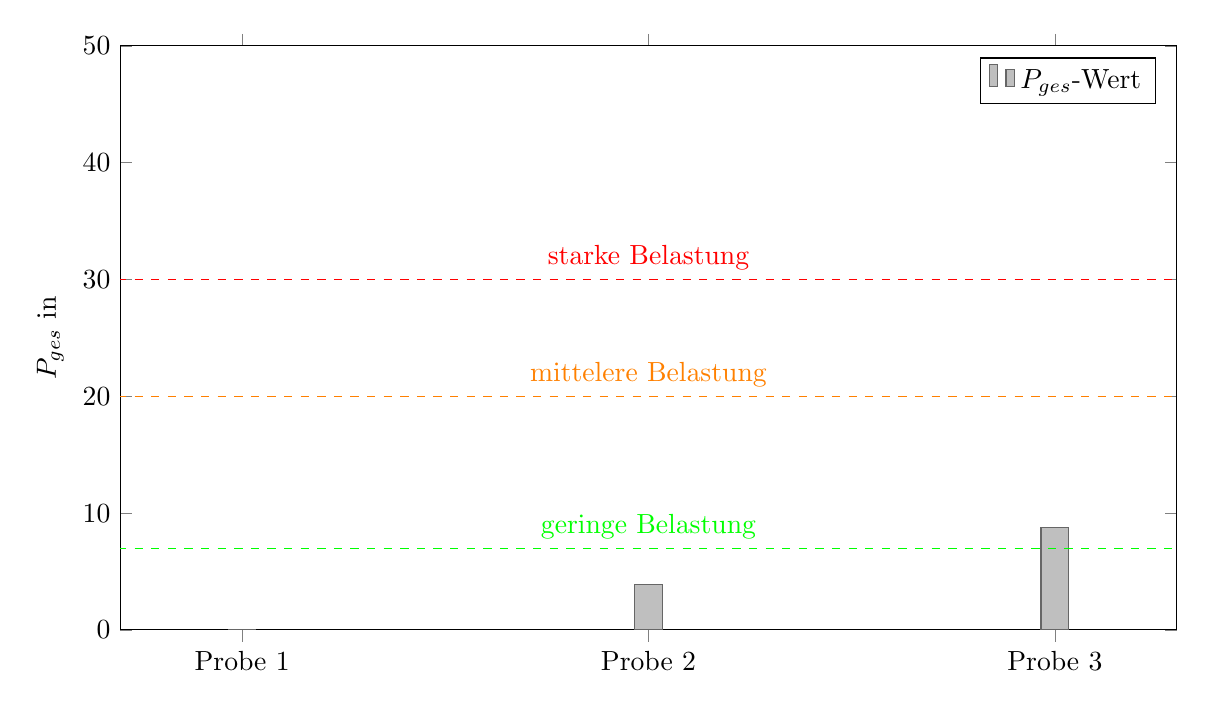
\begin{tikzpicture}
	\begin{axis}[
	%x tick label style={
	%	/pgf/number format/1000 sep=},
	xtick = data,
	ylabel=$P_{ges}$ in \si{\milli \gram \per \liter},
	enlarge x limits=0.15,
	ybar,
	ymin = 0,
	ymax = 50,
	bar width=10pt,
	width=15cm,
	height=9cm,
	symbolic x coords={0,Probe 1, Probe 2,Probe 3,2,1},
	]
	\addplot[fill=gray!50,draw=black!60] coordinates {(Probe 1,0) (Probe 2,3.9) (Probe 3,8.8)};
	\addplot[green,sharp plot,update limits=false, dashed] 
	coordinates {(0,7) (1,7)} 
	node[above] at (axis cs:Probe 2,7) {geringe Belastung};
	\addplot[orange,sharp plot,update limits=false, dashed] 
	coordinates {(0,20) (1,20)} 
	node[above] at (axis cs:Probe 2,20) {mittelere Belastung};
	\addplot[red,sharp plot,update limits=false, dashed] 
	coordinates {(0,30) (1,30)} 
	node[above] at (axis cs:Probe 2,30) {starke Belastung};
	\legend{$P_{ges}$-Wert}
	\end{axis}
	\end{tikzpicture}
	\caption{$P_{ges}$-Beschaffenheit der Abwasserproben 1 bis 3}
	\label{pges}
\end{figure}
\FloatBarrier

